
\appendix
\chapter{Feldbeschreibungen}
\label{app:feldbeschreibungen}
Nachfolgend werden die Felder der Daten beschrieben.

Es gibt dabei folgende Datentypen:
\begin{itemize}
\item integer: geordnete Ganzzahlen $\mathbb{Z}$
\item date: Datum im Format yyyy-mm-dd (y = year, m = month, d = day)
\item categorical: Limitierte Liste von ungeordneten Werten
\item boolean: Attribut kann zwei Werte, "`wahr"' oder "`falsch"', annehmen. 
\item string: Beliebiger ungeordneter Text.
\item float: geordnete reelle Zahl $\mathbb{R}$
\end{itemize}

\rowcolors{1}{tablebodycolor}{tablerowcolor}
\begin{longtable}{ | c | c | c | L{7.5cm} | } 
	\hline 
	\rowcolor{tableheadcolor}
	\bfseries Zelle & \bfseries Name & \bfseries Datentyp & \bfseries Beschreibung \\ \hline 
	
	\rowcolor{tableheadcolor}
	\multicolumn{4}{|c|}{\textbf{Buchungsdaten}} \\ \hline
	A & RESNRDIS & integer & Eindeutige Buchungsnummer \\ \hline 
	B & RESINSDATE & date & Erstellungsdatum der Buchung \\ \hline 
	C & BOOKSTA & categorical & Status der Buchung \\ \hline 
	D & SELCURR & categorical & Währung \\ \hline 
	E & PRICES & integer & Preis \\ \hline 
	F & SONR & categorical & Sales Office Nummer \\ \hline 
	G & MAINSONR & categorical & Main Sales Office Nummer \\ \hline 
	H & BOOKLANG & categorical & Sprache der Benutzers \\ \hline 
	I & NREF & categorical & Nummer des gebuchten Objekts \\ \hline 
	J & RESBEGDATE & date & Startdatum des Aufenthaltes \\ \hline 
	K & RESENDDATE & date & Enddatum des Aufenthaltes \\ \hline 
	L & REPAX & integer & Anzahl Passagiere \\ \hline 
	M & READULT & integer & Anzahl Erwachsene \\ \hline 
	N & RECHILD & integer & Anzahl Kinder \\ \hline 
	O & REBABY & integer & Anzahl Babies \\ \hline 
	P & CUTITLE & categorical & Anrede des Kunden \\ \hline 
	Q & CUNAME & string & Name des Kunden \\ \hline 
	R & CUSTRAS & string & Strasse des Kunden \\ \hline 
	S & CUCNTRY & categorical & Land des Kunden \\ \hline 
	T & CUZIP & integer & Postleitzahl des Kunden \\ \hline 
	U & CUORT & string & Ortschaft des Kunden \\ \hline 
	
	\rowcolor{tableheadcolor}
	\multicolumn{4}{|c|}{\textbf{Objektdaten}} \\ \hline
	V & OBGEOLAT & float & Breitengrad des Objekts \\ \hline 
	W & OBGEOLONG & float & Längengrad des Objekts \\ \hline 
	X & OBSTRAS & string & Strasse des Objekts \\ \hline 
	Y & OBCNTRY & categorical & Land des Objekts \\ \hline 
	Z & OBZIP & integer & Postleitzahl des Objekts \\ \hline 
	AA & OBORT & string & Ortschaft des Objekts \\ \hline 
	AB & PAX & string & Anzahl möglicher Gäste \\ \hline 
	AC & QUAL & string & Sterne Bewertung des Objekts \\ \hline 
	AD & ROOMS & string & Anzahl Zimmer \\ \hline 
	AE & BEDROOMS & string & Anzahl Schlafzimmer \\ \hline 
	AF & BRAND & categorical & Provider des Objekts. A = Villa Vacant, B = Bungalow.Net, C = Interchalet, DAC = Dan Center, D = Sol og Strang, E = DanCenter, F = Belvilla, FER = Feratel, G = Adagio, H = Hotelpac, I = Interhome, J = Just France, JAS = Jassu Travel, L = Lomarengas, M = HR Special Residence, NFM = Norddeich Ferienwohnungen Maus GmbH, O = Roompot, P = Topic Travel, Q = Aquadelta, R = Resortquest, S = TOMAS, T = Tui Wolters, V = Vacando, W = PO for IH, Y = Centerparcs, Z = Sunpars, IL = Interhome Light, TAB = Total Accommodation Booking System, APA = Apartments Apart, PVI = Portvil, AMA = Interhome, SPR = Swisspeak Resorts\\ \hline 
	AG & ACCOMTYPE & categorical & Typ des Objekts\\ \hline 
	AH & PETS & boolean & Haustiere erlaubt? \\ \hline 
	AI & CHOUSE & categorical & A = Apartment (Wohnung), H = ) \\ \hline 
	AJ & HOUSETYPE & categorical & Typ des Hauses ??? \\ \hline 
	AK & DIWATER & integer & Distanz zum Wasser (m) \\ \hline 
	AL & DISKI & integer & Distanz zum Skigebiet (m) \\ \hline 
	AM & DIPUBT & integer & Distanz zum öffentlichen Verkehr (m) \\ \hline 
	AN & DIGOLF & integer & Distanz zum Golfplatz (m) \\ \hline 
	AO & CNATURE & boolean & Naturbelassene Umgebung \\ \hline 
	AP & CTRANQUILI & boolean & Ruhige Umgebung \\ \hline 
	AQ & CBATHANDSH & boolean & Bad oder eine Dusche im Objekt \\ \hline 
	AR & CAIRCOND & boolean & Aircondition im Objekt\\ \hline 
	AS & CCENTRAL & boolean & Objekt liegt zentral gelegen \\ \hline 
	AT & CSUNNY & boolean & Umgebung des Objekts ist sonnig \\ \hline 
	AU & CFENCED & boolean & Objekt ist umzäunt \\ \hline 
	AV & CGARDEN & boolean & Objekt besitzt einen Garten \\ \hline 
	AW & CPOOL & boolean & Objekt besitzt einen Pool \\ \hline 
	AX & CPPOOL & boolean & Objekt besitzt einen privaten Pool \\ \hline 
	AY & CHEATED & boolean & Objekt besitzt einen geheizten Pool \\ \hline 
	AZ & CSAFEPOOL & boolean & Objekt besitzt einen sicheren Pool \\ \hline 
	BA & CCHILDPOOL & boolean & Objekt besitzt einen kindersicheren Pool \\ \hline 
	BB & CTENNIS & boolean & Objekt besitzt einen Tennisplatz \\ \hline 
	BC & CBBQ & boolean & Objekt besitzt einen Grill \\ \hline 
	BD & CRECEPTION & boolean & Objekt besitzt eine Rezeption \\ \hline 
	BE & CRESTAURAN & boolean & Objekt besitzt ein Restaurant \\ \hline 
	BF & CSAUNA & boolean & Objekt besitzt eine Saune \\ \hline 
	BG & CFITNESS & boolean & Objekt besitzt ein Fitness \\ \hline 
	BH & CMASSAGE & boolean & Massagen können bezogen werden \\ \hline 
	BI & CJACUZZI & boolean & Objekt besitzt ein Jacuzzi \\ \hline 
	BJ & CBILLARD & boolean & Objekt besitzt einen Billiardtisch \\ \hline 
	BK & CTABLETENN & boolean & Objekt besitzt einen Tischtennis Tisch \\ \hline 
	BL & CELEVATOR & boolean & Objekt besitzt einen Lift \\ \hline 
	BM & CWASHMACHI & boolean & Objekt besitzt eine Waschmaschine \\ \hline 
	BN & CDRYER & boolean & Objekt besitzt einen Trockner \\ \hline 
	BO & CCHANGELIN & boolean & Es gibt einen Service um die Bettwäsche zu wechseln \\ \hline 
	BP & CCLEANING & boolean & Es gibt einen Reinigungsservice \\ \hline 
	BQ & CMAIDENSER & boolean & Es gibt einen Aufräumservice \\ \hline 
	BR & CFRESHBREA & boolean & Frisches Brot kann in nächster Umgebung bezogen werden \\ \hline 
	BS & CBREAKFAST & boolean & Es kann in nächster Umgebung gefrühstückt werden \\ \hline 
	BT & CHALFBOARD & boolean & Es wird halbpension angeboten \\ \hline 
	BU & CPARKING & boolean & Es gibt einen Parkplatz \\ \hline 
	BV & CDISHWASHE & boolean & Objekt besitzt einen Geschirrspühler \\ \hline 
	BW & CFIREPLACE & boolean & Objekt besitzt ein Cheminée \\ \hline 
	BX & SCTV & boolean & Objekt besitzt einen Fernseher \\ \hline 
	BY & SCBALCONY & boolean & Objekt besitzt ein Balkon \\ \hline 
	BZ & SCFREEZER & boolean & Objekt besitzt einen Tiefkühler \\ \hline 
	CA & SCNOSMOKE & boolean & Im Objekt darf nicht geraucht werden \\ \hline 
	CB & CSNATURECO & boolean & Naturbelassene Umgebung im Sommer \\ \hline 
	CC & CWNATURECO & boolean & Naturbelassene Umgebung im Winter \\ \hline 
	CD & CBATHSEA & boolean & In der Umgebung kann im Mehr gebadet werden \\ \hline 
	CE & CBATHLAKE & boolean & In der Umgebung kann in einem See gebadet werden \\ \hline 
	CF & CMOUNTLAKE & boolean & In der Umgebung kann in einem Bergsee gebadet werden \\ \hline 
	CG & CSRESTRELA & boolean & ??? \\ \hline 
	CH & CWRESTRELA & boolean & ??? \\ \hline 
	CI & CMETROPOLI & boolean & Objekt liegt in einer Metropole \\ \hline 
	CJ & CHIKINGMOU & boolean & In der Umgebung kann kann in den Bergen gewandert werden \\ \hline 
	CK & CHIKINGPLA & boolean & In der Umgebung kann  \\ \hline 
	CL & CNORDICWAL & boolean & In der Umgebung kann im Flachland gewandert werden \\ \hline 
	CM & CSACTFUNSP & boolean & In der Umgebung kann im Sommer Aktivsport betrieben werden \\ \hline 
	CN & CWACTFUNSP & boolean & In der Umgebung kann im Winter Aktivsport betrieben werden \\ \hline 
	CO & CENTERPARK & boolean & In der Umgebung kann gibt es ein Vergnügungspark \\ \hline 
	CP & CBIKINGMOU & boolean & In der Umgebung kann in den Bergen Fahrrad gefahren werden \\ \hline 
	CQ & CBIKINGPLA & boolean & In der Umgebung kann im Flachland Fahrrad gefahren werden \\ \hline 
	CR & CSAILING & boolean & In der Umgebung kann kann gesegelt werden \\ \hline 
	CS & CSURFING & boolean & In der Umgebung kann man surfen \\ \hline 
	CT & CWINDSURF & boolean & In der Umgebung kann windsurfen \\ \hline 
	CU & CSNIGHTLIF & boolean & In der Umgebung gibt es Nachtleben im Sommer \\ \hline 
	CV & CWNIGHTLIF & boolean & In der Umgebung gibt es Nachtlegen im Winter \\ \hline 
	CW & CSSENIOR & boolean & Objekt ist im Sommer seniorentauglich \\ \hline 
	CX & CWSENIOR & boolean & Objekt ist im Winter seniorentauglich \\ \hline 
	CY & CSFAMILY & boolean & Objekt ist im Sommer familientauglich \\ \hline 
	CZ & CWFAMILY & boolean & Objekt ist im Winter familientauglich \\ \hline 
	DA & CSIDYLIC & boolean & Objekt ist im Sommer idyllisch \\ \hline 
	DB & CWIDYLIC & boolean & Objekt ist im Winter idyllisch \\ \hline 
	DC & CHISTORIC & boolean & Objekt liegt in einer historischen Umgebung \\ \hline 
	DD & CWINEDINE & boolean & ??? \\ \hline 
	DE & CSUITHOMO & boolean & ??? \\ \hline 
	DF & CTYPVILLAG & boolean & Objekt liegt in einem Dorf \\ \hline 
	DG & CCOVERPARK & boolean & ??? \\ \hline 
	DH & CTYPRUSTIC & boolean & Objekt ist rustikal eingerichtet \\ \hline 
	DI & CTYPCOMFOR & boolean & Objekt ist konfortabel eingerichtet \\ \hline 
	DJ & CTYPLUXUR & boolean & Objekt ist luxuriös eingerichtet \\ \hline 
	DK & CTYPMODERN & boolean & Objekt ist modern eingerichtet \\ \hline 
	DL & CTYPHISTOR & boolean & Objekt ist historisch eingerichtet \\ \hline 
	DM & AIRPORT1 & categorical & IATA Code des nächsten Flughafen \\ \hline 
	DN & DIAIRPORT1 & integer & Distanz bis zum nächsten Flughafen (km) \\ \hline 
	DO & CROSSSKIIN & boolean & In der Umgebung kann Crossski gefahren werden \\ \hline 
	DP & ICERINK & boolean & In der Umgebung gibt es eine Eisbahn \\ \hline 
	DQ & SKIAREA & boolean & In der Umgebung gibt es ein Skigebiet \\ \hline 
	DR & SNOWBOARD & boolean & In der Umgebung kann Snowboard gefahren werden \\ \hline 
	DS & TOBOGGAN & boolean & In der Umgebung kann man Rodeln \\ \hline 
	DT & WINTERWALK & boolean & In der Umgebung kann man im Winter wandern \\ \hline 
	DU & OUTDPOOL & categorical & Objekt besitzt einen aussen Pool \\ \hline 
	DV & INDPOOL & boolean & Objekt besitzt einen innen Pool \\ \hline 
	DW & DVDPLAYER & boolean & Objekt besitzt einen DVD Player \\ \hline 
	DX & PTENNIS & boolean & Objekt besitzt einen privaten Tennisplatz \\ \hline 
	DY & SOLARIUM & boolean & Objekt besitzt ein Solarium \\ \hline 
	DZ & DICENTER & integer & Distanz bis zum Zentrum (m) \\ \hline 
	EA & DISEA & integer & Distanz bis zum Meer (m) \\ \hline 
	EB & DILAKE & integer & Distanz bis zum See (m) \\ \hline 
	EC & CRESIDENCE & boolean & Objekt ist eine Residenz \\ \hline 
	ED & CPTENNIS & boolean & Objekt besitzt einen privaten Tennisplatz \\ \hline 
	EE & CHORSE & boolean & In der Umgebung kann man reiten \\ \hline 
	EF & CVIEWSEA & boolean & Objekt besitzt eine Aussicht auf das Meer \\ \hline 
	EG & INTERNET & boolean & Objekt besitzt Internet \\ \hline 
	EH & CHILDPGRND & boolean & Objekt besitzt einen Kinderspielplatz \\ \hline 
	EI & CISLAND & boolean & Objekt liegt auf einer Insel \\ \hline 
	EJ & CVIEWMOUNT & boolean & Objekt besitzt eine Aussicht auf die Berge \\ \hline 
	EK & CVIEWCNTRY & boolean & Objekt besitzt eine Aussicht auf das Flachland \\ \hline 
	EL & CVIEWLAKE & boolean & Objekt besitzt eine Aussicht auf einen See \\ \hline 
	EM & CBATH & boolean & Objekt besitzt ein Bad \\ \hline 
	EN & CSHOWER & boolean & Objekt besitzt eine Dusche \\ \hline 
	EO & CCARPORT & boolean & ??? \\ \hline 
	EP & CSGARAGE & boolean & ??? \\ \hline 
	EQ & CCGARAGE & boolean & ??? \\ \hline 
	ER & CGOLFCOURS & boolean & In der Umgebung gibt es einen Golfplatz \\ \hline 
	ES & CWELLNESS & boolean & In der Umgebung gibt es ein Wellness \\ \hline 
	ET & CMICROWAVE & boolean & Objekt besitzt eine Mikrowelle \\ \hline 
	EU & COVEN & boolean & Objekt besitzt einen Ofen \\ \hline 
	EV & CPHONE & boolean & Objekt besitzt ein Telefon \\ \hline 
	EW & CTERRACE & boolean & Objekt besitzt eine Terasse \\ \hline 
	\caption{Attributbeschreibung}
\end{longtable} 

\chapter{Testdatenquellen}
\label{app:testdatenquellen}

%\num[round-mode=places,round-precision=7]{}
\csvstyle{myTableStyle}{tabular=|c|c||c|c|c|c|c|c||c|c|,
	separator=semicolon,
	table head=\hline \rowcolor{tableheadcolor} \multicolumn{2}{|c||}{General} & \multicolumn{6}{c||}{Categorical} & \multicolumn{2}{c|}{Numerical} \\\hline
	\rowcolor{tableheadcolor} \rotatebox{90}{id} & \rotatebox{90}{NREF} & \rotatebox{90}{Distanz zum Wasser} & \rotatebox{90}{Distanz zum ÖV} & \rotatebox{90}{Distanz zum Meer} & \rotatebox{90}{Wochenpreis} & \rotatebox{90}{Haustiere erlaubt} & \rotatebox{90}{Aircondition vorhanden} & \rotatebox{90}{Anzahl Zimmer} & \rotatebox{90}{Anzahl Schlafzimmer} \\ ,
	late after line=\\,
	late after last line=\\\hline,
	head to column names}


\section{TC1: 2 gleiche Distanzattribute}
\label{app:testdatenquellen:1}

\csvreader[myTableStyle]%
{testcases/data-apriori-2-entries--2-distances.csv}
{}
{\id & \NREF & \DIWATER & \DIPUBT & \DISEA & \weeklyprice & \PETS & \CAIRCOND & \ROOMS & \BEDROOMS}

\section{TC2: 2 gleiche Binärattribute}
\label{app:testdatenquellen:2}

\csvreader[myTableStyle]%
{testcases/data-apriori-2-entries--2-binary-attributes.csv}
{}
{\id & \NREF & \DIWATER & \DIPUBT & \DISEA & \weeklyprice & \PETS & \CAIRCOND & \ROOMS & \BEDROOMS}

\section{TC3: 2 gleiche numerische Attribute}
\label{app:testdatenquellen:3}

\csvreader[myTableStyle]%
{testcases/data-apriori-2-entries--2-numeric-attributes.csv}
{}
{\id & \NREF & \DIWATER & \DIPUBT & \DISEA & \weeklyprice & \PETS & \CAIRCOND & \ROOMS & \BEDROOMS}

\section{TC4: 1 numerisches und 1 Binärattribut}
\label{app:testdatenquellen:4}

\csvreader[myTableStyle]%
{testcases/data-apriori-2-entries--1-numeric-1-binary-attribute.csv}
{}
{\id & \NREF & \DIWATER & \DIPUBT & \DISEA & \weeklyprice & \PETS & \CAIRCOND & \ROOMS & \BEDROOMS}

\section{TC5: 2 gleiche Distanzattribute mit einem Binärfilter}
\label{app:testdatenquellen:5}

\csvreader[myTableStyle]%
{testcases/data-apriori-2-entries--binary-filter--2-distances.csv}
{}
{\id & \NREF & \DIWATER & \DIPUBT & \DISEA & \weeklyprice & \PETS & \CAIRCOND & \ROOMS & \BEDROOMS}

\section{TC6: 2 gleiche Distanzattribute mit einem Distanzfilter}
\label{app:testdatenquellen:6}

\csvreader[myTableStyle]%
{testcases/data-apriori-2-entries--distance-filter--2-distances.csv}
{}
{\id & \NREF & \DIWATER & \DIPUBT & \DISEA & \weeklyprice & \PETS & \CAIRCOND & \ROOMS & \BEDROOMS}

\section{TC7: 2 gleiche Distanzattribute mit einem numerischen Filter}
\label{app:testdatenquellen:7}

\csvreader[myTableStyle]%
{testcases/data-apriori-2-entries--number-filter--2-distances.csv}
{}
{\id & \NREF & \DIWATER & \DIPUBT & \DISEA & \weeklyprice & \PETS & \CAIRCOND & \ROOMS & \BEDROOMS}

\section{TC8: 2 gleiche Distanz- und 1 binäres Attribut}
\label{app:testdatenquellen:8}

\csvreader[myTableStyle]%
{testcases/data-apriori-3-entries--2-distances-1-binary.csv}
{}
{\id & \NREF & \DIWATER & \DIPUBT & \DISEA & \weeklyprice & \PETS & \CAIRCOND & \ROOMS & \BEDROOMS}

\section{TC9: Zwei Menten mit einmal 2 Distanzen und einmal 1 numerischen und 1 Binärattritbut}
\label{app:testdatenquellen:9}

\csvreader[myTableStyle]%
{testcases/data-apriori-3-entries-two-sets--2-distances--1-number-1-binary.csv}
{}
{\id & \NREF & \DIWATER & \DIPUBT & \DISEA & \weeklyprice & \PETS & \CAIRCOND & \ROOMS & \BEDROOMS}

\section{TC10: 2 Clusters mit jeweils 5 Elementen}
\label{app:testdatenquellen:10}

\csvreader[myTableStyle]%
{testcases/data-cluster-2-entries--2-clusters--5-and-5--0-distance.csv}
{}
{\id & \NREF & \DIWATER & \DIPUBT & \DISEA & \weeklyprice & \PETS & \CAIRCOND & \ROOMS & \BEDROOMS}

\section{TC11: 1 Cluster mit 1 Element und 1 Cluster mit 9 Elementen}
\label{app:testdatenquellen:11}

\csvreader[myTableStyle]%
{testcases/data-cluster-2-entries--2-clusters--9-and-1--0-distance.csv}
{}
{\id & \NREF & \DIWATER & \DIPUBT & \DISEA & \weeklyprice & \PETS & \CAIRCOND & \ROOMS & \BEDROOMS}

\section{TC12: 2 Cluster mit kleinen Unterschieden}
\label{app:testdatenquellen:12}

\csvreader[myTableStyle]%
{testcases/data-cluster-minor-differences-2-entries--2-clusters--5-and-5--0-distance.csv}
{}
{\id & \NREF & \DIWATER & \DIPUBT & \DISEA & \weeklyprice & \PETS & \CAIRCOND & \ROOMS & \BEDROOMS}



\chapter{Klassendiagramme}
\label{app:klassendiagram}
Nachfolgend werden die Klassendiagramme präsentiert. Die Erklärung dazu ist im \cref{sec:proofofconcept:klassenstruktur} zu finden.
\begin{figure}[H]
	\centering
	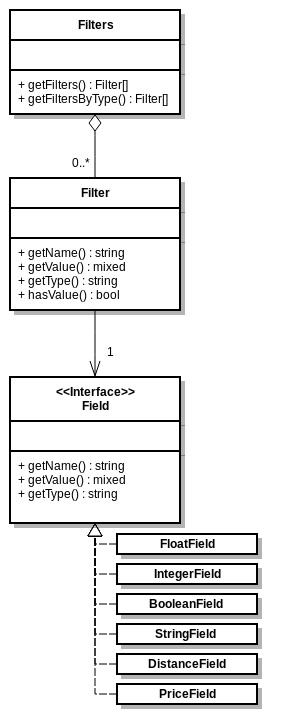
\includegraphics[width=0.5\textwidth]{images/diagram-class-filters}
	\caption{Klassendiagramm der Filter und Felder Datenmodelle}
	\label{fig:proofofconcept:klassenstruktur:5}
\end{figure}
\begin{figure}[H]
	\centering
	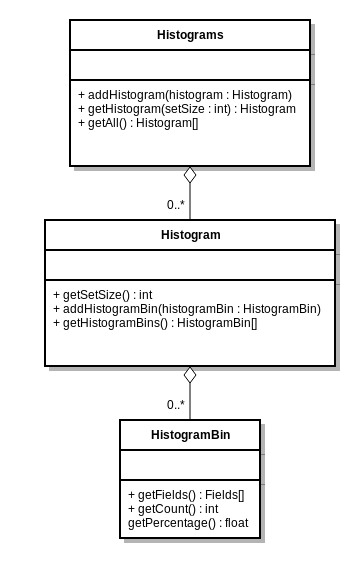
\includegraphics[width=0.6\textwidth]{images/diagram-class-Histograms}
	\caption{Klassendiagramm der Histogram-Modelle}
	\label{fig:proofofconcept:klassenstruktur:6}
\end{figure}
\begin{sidewaysfigure}[H]
	\centering
	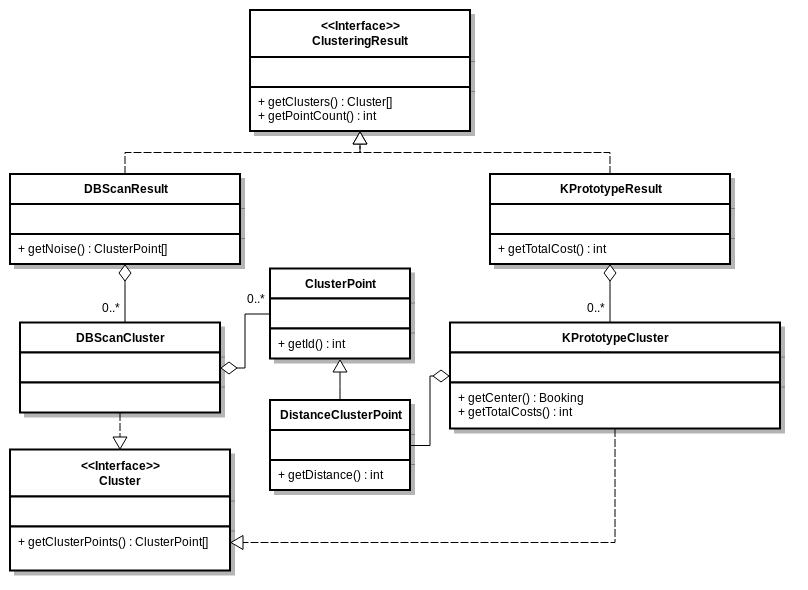
\includegraphics[width=1\textwidth]{images/diagram-class-clusters}
	\caption{Klassendiagramm der Clusterresultate}
	\label{fig:proofofconcept:klassenstruktur:7}
\end{sidewaysfigure}
\begin{figure}[H]
	\centering
	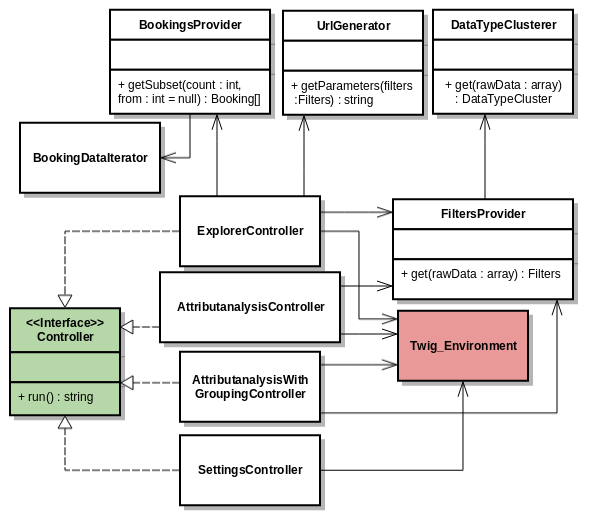
\includegraphics[width=1\textwidth]{images/diagram-class-Controller}
	\caption{Klassendiagramm der Controller}
	\label{fig:proofofconcept:klassenstruktur:1}
\end{figure}
\begin{sidewaysfigure}[H]
	\centering
	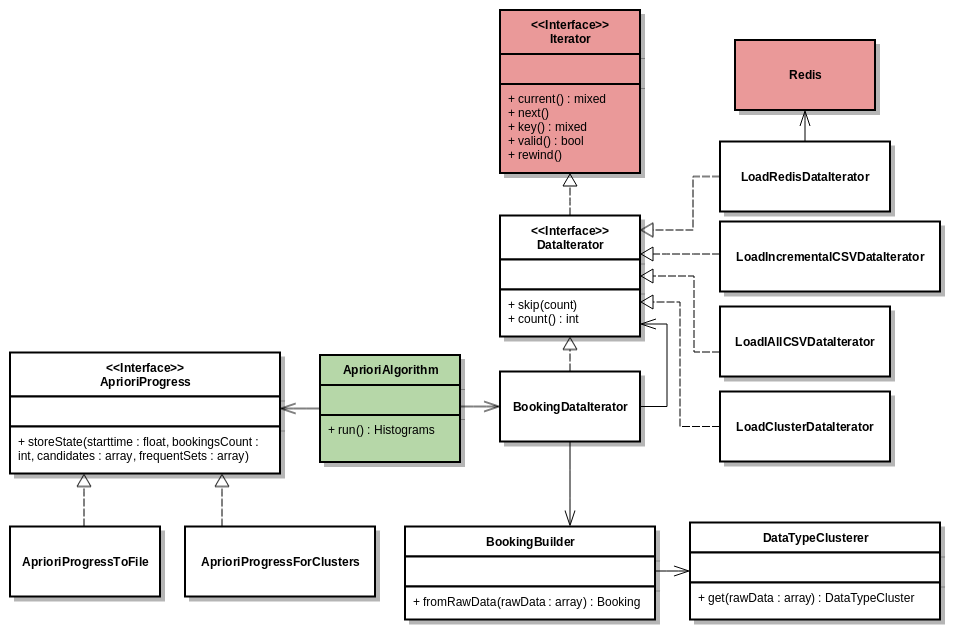
\includegraphics[width=1\textwidth]{images/diagram-class-AprioriAlgorithm}
	\caption{Klassendiagramm des Apriori Alogorithmus}
	\label{fig:proofofconcept:klassenstruktur:2}
\end{sidewaysfigure}
\begin{figure}[H]
	\centering
	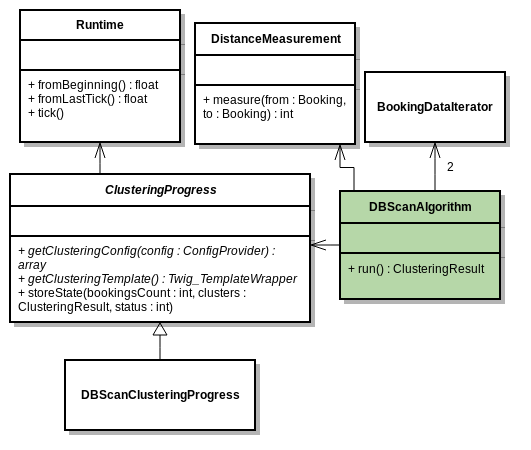
\includegraphics[width=1\textwidth]{images/diagram-class-DBScanAlgorithm}
	\caption{Klassendiagramm des DBScan Alogorithmus}
	\label{fig:proofofconcept:klassenstruktur:3}
\end{figure}
\begin{figure}[H]
	\centering
	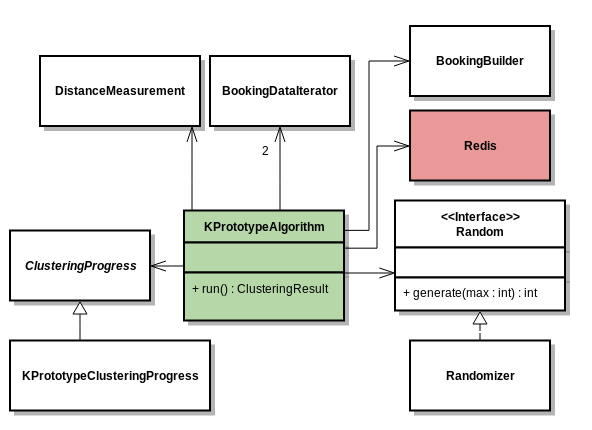
\includegraphics[width=1\textwidth]{images/diagram-class-KPrototypeAlgorithm}
	\caption{Klassendiagramm des KPrototype Alogorithmus}
	\label{fig:proofofconcept:klassenstruktur:4}
\end{figure}

\chapter{Ansichten des Programms}
Nachfolgend werden Ansichten des Programms aufgezeigt, die in der Proof of Concept Phase umgesetzt wurden.
\label{app:pocansichten}
\begin{figure}[H]
	\RawFloats
	\centering
	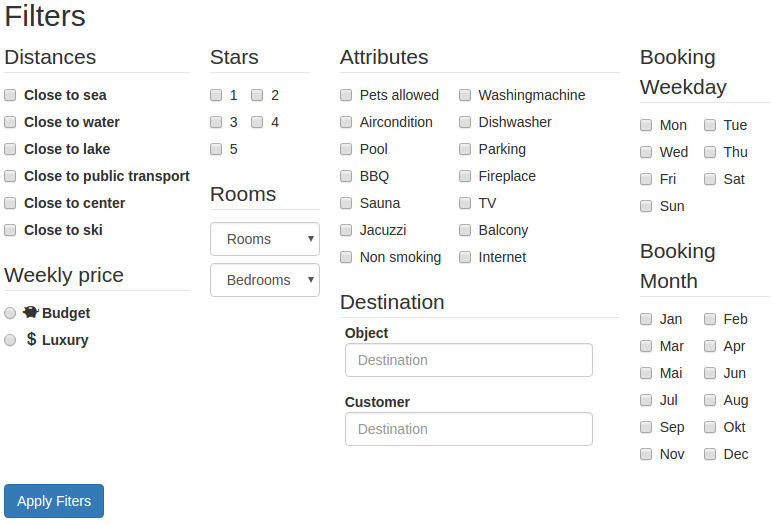
\includegraphics[width=1\textwidth]{images/program-filters}
	\caption{Ansichten des Programms: Filters}
\end{figure}
\begin{figure}[H]
	\RawFloats
	\centering
	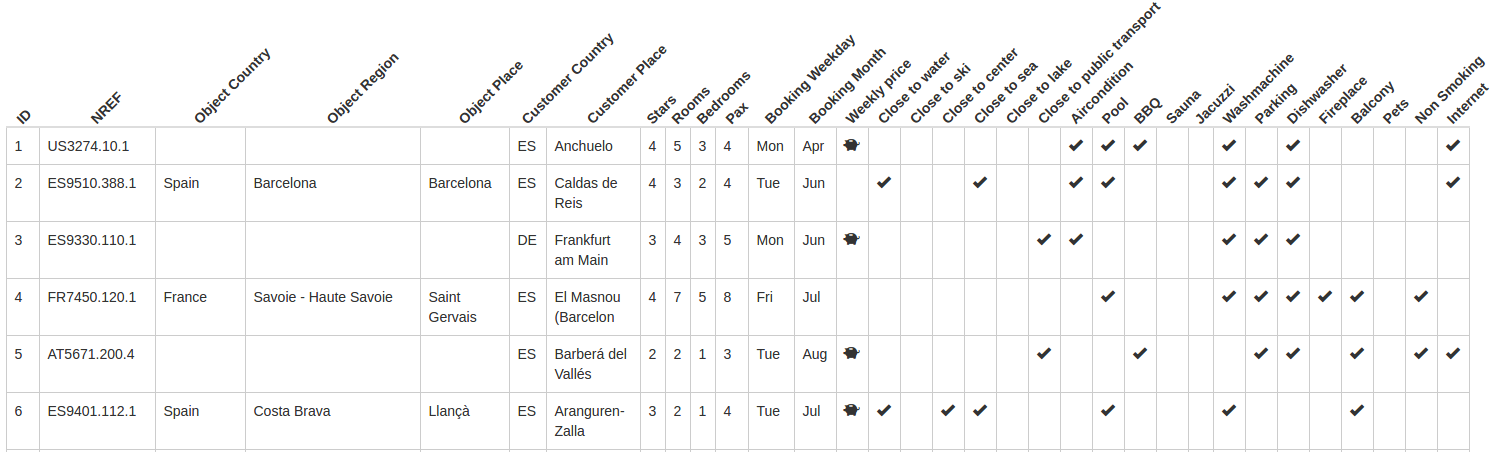
\includegraphics[width=1\textwidth]{images/program-explore-results}
	\caption{Ansichten des Programms: Stammdaten einsehen}
\end{figure}
\begin{figure}[H]
	\RawFloats
	\centering
	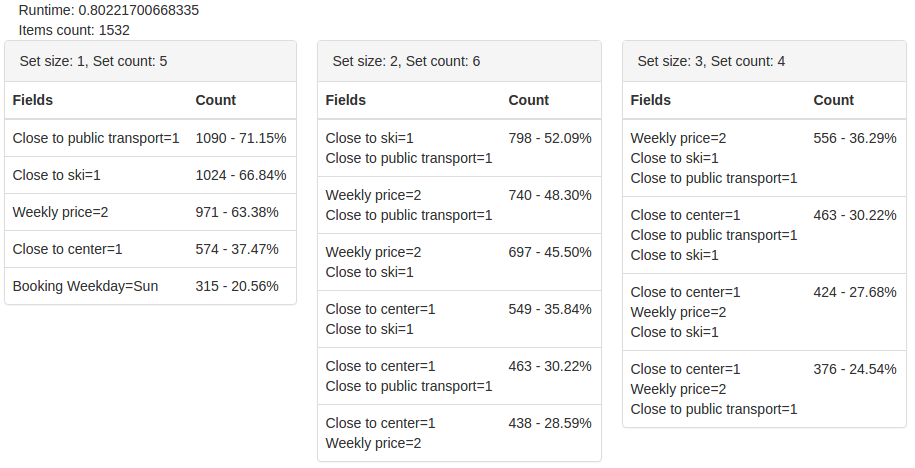
\includegraphics[width=1\textwidth]{images/program-apriori-results}
	\caption{Ansichten des Programms: Resultat einer Apriori Analyse}
\end{figure}
\begin{figure}[H]
	\RawFloats
	\centering
	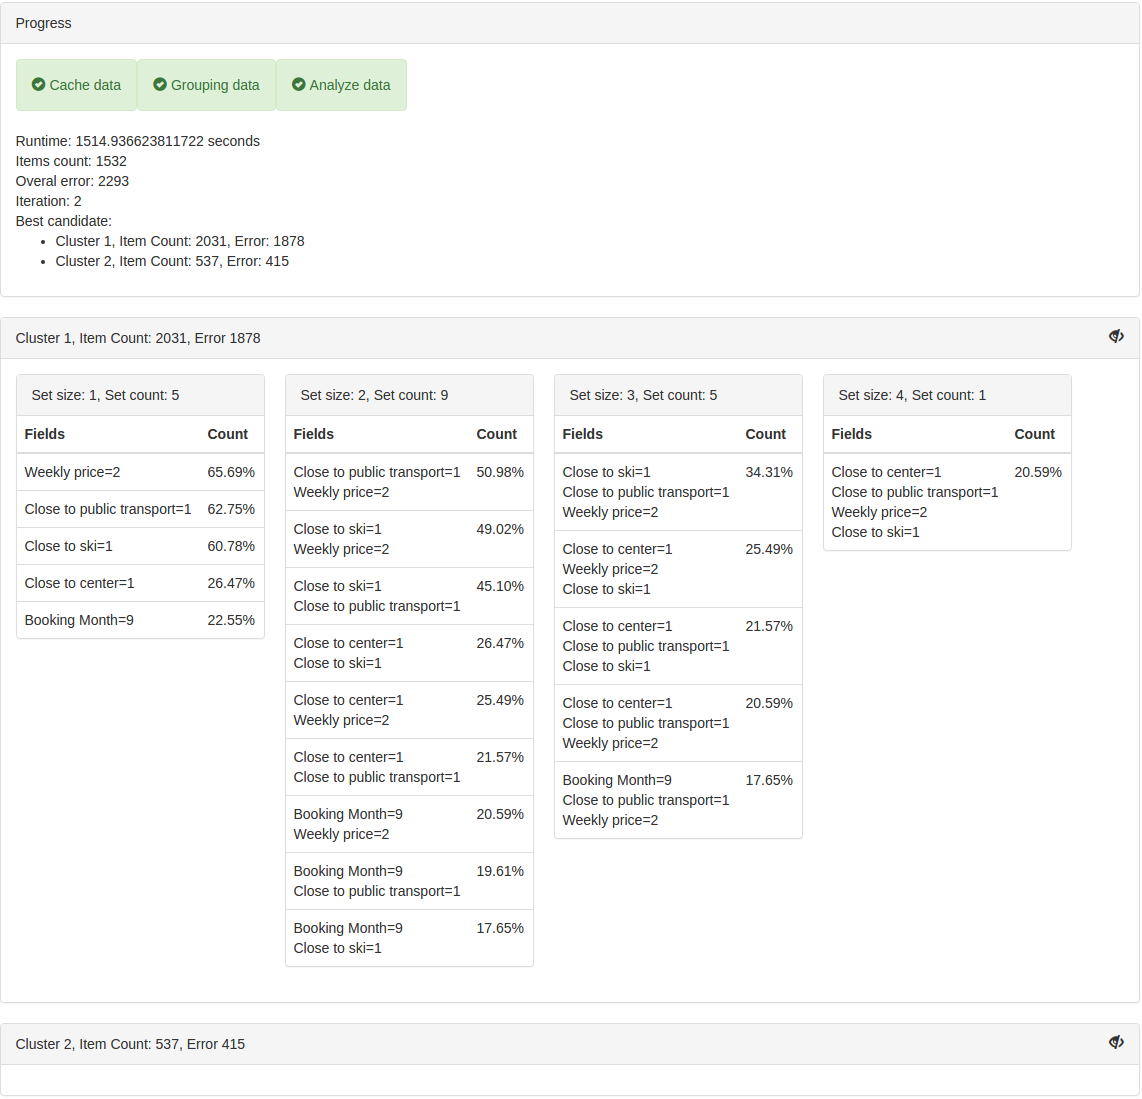
\includegraphics[width=1\textwidth]{images/program-kprototype-results}
	\caption{Ansichten des Programms: Resultat einer k-prototype Analyse}
\end{figure}
\begin{figure}[H]
	\RawFloats
	\centering
	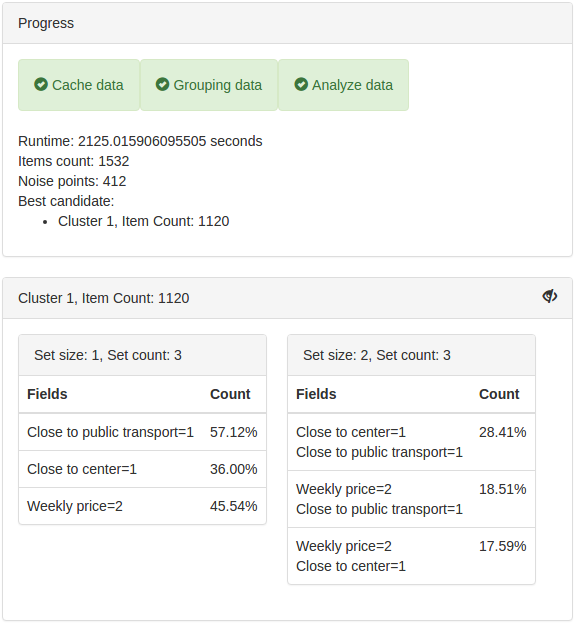
\includegraphics[width=0.8\textwidth]{images/program-dbscan-results}
	\caption{Ansichten des Programms: Resultat einer DBSCAN Analyse}
\end{figure}
\begin{figure}[H]
	\RawFloats
	\centering
	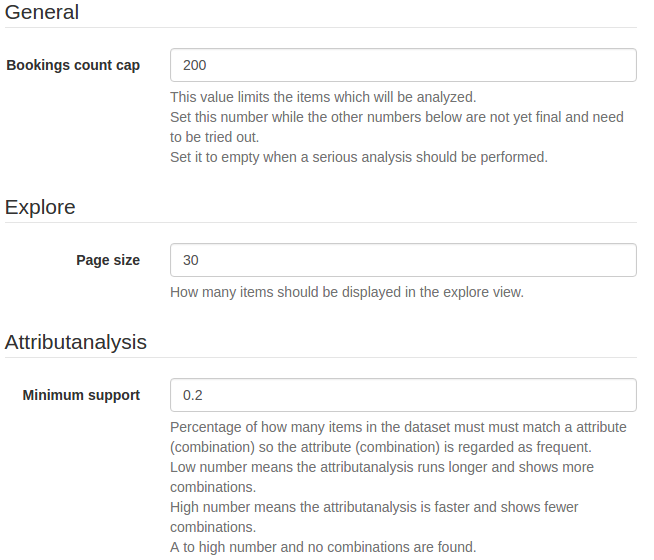
\includegraphics[width=1\textwidth]{images/program-settings}
	\caption{Ansichten des \textbf{Programms}: Ausschnitt der Ansicht "`Algorithmen konfigurieren"'}
\end{figure}
